\chapter{Methodology and Concept Development}
\label{chap:methodology}

This chapter presents the systematic approach taken in designing the \ac{VMAP} system. The methodology follows established software engineering principles to address the complex requirements of automotive parameter management. Beginning with a requirements analysis, the chapter proceeds to detail the conceptual architecture design, data model, validation mechanisms, and integration approaches developed to ensure system robustness and compatibility with existing enterprise infrastructure.

\section{Requirements Analysis}
\label{sec:requirements-analysis}

The foundation of the \ac{VMAP} system design was a comprehensive requirements analysis conducted through structured interviews with stakeholders, detailed examination of the existing Excel-based process, and workshops with domain experts. This multi-faceted approach, following Hull's framework for requirements engineering, ensured that both functional and non-functional requirements would be thoroughly identified and prioritized \cite{hull2010requirements}.

\subsection{Functional Requirements}
\label{subsec:functional-requirements}

The primary functional requirements were derived from direct observation of engineers' current Excel-based workflow combined with semi-structured interviews conducted with module developers and documentation specialists. The system must support the hierarchical organization of parameters within \acp{ECU}, Modules, and \acp{PID}, mirroring the domain-specific structure of automotive electronic systems as described by Staron \cite{staron2021automotive}. This hierarchical organization is essential for maintaining the logical structure of vehicle parameters and aligning with established engineering practices.

Users must be able to create variants for parameters with specific code rules determining their applicability, and define segments representing modified parameter values. If no segment exists, the system must default to Parameter Definition Database values—an approach that allows efficient storage by tracking only modifications rather than duplicating unchanged parameters, aligning with Bhattacherjee's principles of dataset versioning \cite{bhattacherjee2015principles}.

The system must track parameter values across four distinct release phases: Phase1, Phase2, Phase3, and Phase4, with changes in earlier phases propagating to later phases unless explicitly overridden. This phase-based approach represents a domain-specific adaptation particularly suited to automotive software development cycles as identified in Broy's research on automotive software engineering challenges \cite{broy2006challenges}.

All modifications require comprehensive logging with user information, timestamp, and detailed change data, supporting regulatory compliance and enabling parameter evolution tracking. The system must also provide functionality to create parameter configuration snapshots at specific points, particularly at phase transitions, for documentation purposes—a capability identified as essential for quality assurance and regulatory compliance in automotive software development by Staron \cite{staron2021automotive}.

\subsection{Integration with External Systems}
\label{subsec:integration-external-systems}

The stakeholder interviews and process analysis revealed that \ac{VMAP} must integrate with two critical external enterprise systems: the \ac{PDD} and the \ac{VCD}. The \ac{PDD} serves as the authoritative source for the hierarchical structure of automotive electronic systems, containing definitions of \acp{ECU}, Modules, \acp{PID}, and baseline parameter configurations. As noted by Pretschner et al. \cite{pretschner2007software}, maintaining this hierarchical structure is essential for automotive software development.

The \ac{VCD} contains comprehensive vehicle specifications and configuration codes that determine which parameter variants apply to specific vehicle configurations. Integration with this system is necessary for validating the boolean code rules associated with parameter variants and supporting parameter file generation for specific vehicle configurations by resolving the applicable parameter variants based on vehicle codes. This integration requirement aligns with Staron's analysis of automotive software architectures, which emphasizes the importance of configuration management in supporting variant-rich vehicle platforms \cite{staron2021automotive}.

\subsection{User Role Requirements}
\label{subsec:user-role-requirements}

A systematic analysis of the current Excel-based workflow, coupled with contextual inquiries with engineering teams, identified four distinct user roles with specific access requirements. Module developers require write access to parameters within their assigned modules, with the ability to create and modify variants and segments. Documentation specialists need access to frozen data for documentation, comparison capabilities between phases, and comprehensive change history access. System administrators require comprehensive control over user management, release phases, and special operations like variant deletion and phase freezing. Read-only users need view access to all parameter data with parameter file generation capabilities but no modification rights.

These roles were defined based on the principle of least privilege as described by Sandhu \cite{sandhu1998role}, ensuring users have access only to functionality required for their specific responsibilities while enhancing system security and simplifying the user experience.

\subsection{Data Management Requirements}
\label{subsec:data-management-requirements}

The system must maintain distinct parameter versions across different release phases, allowing simultaneous work on multiple phases while enabling access to parameter values from any point in the development lifecycle. As highlighted by Sciore \cite{sciore2009database}, data integrity requires maintaining referential integrity across all related entities, particularly ensuring variants and segments associate with valid parameters.

Multi-dimensional parameter support is essential for complex automotive parameters such as mapping tables. Operations modifying multiple related entities must function as atomic transactions to maintain data consistency—particularly important for phase transitions where numerous parameters, variants, and segments may change simultaneously, a requirement that aligns with Bhattacherjee's research on dataset versioning approaches \cite{bhattacherjee2015principles}.

Query performance analysis, based on projected usage patterns from the current Excel-based process, identified critical query paths including parameter retrieval by \ac{ECU}, module, \ac{PID}, release phase, and parameter name. These requirements influenced schema design decisions regarding normalization and indexing strategies to optimize common query patterns.

\section{Use Case Modeling}
\label{sec:use-case-modeling}

Following the requirements gathering process, use case modeling was employed to formalize the system's functional requirements from a user perspective. This approach, as described by Jacobson \cite{jacobson2004use}, provides a structured way to represent the system's capabilities and the interactions between users and the system.

\begin{figure}[h]
    \centering
    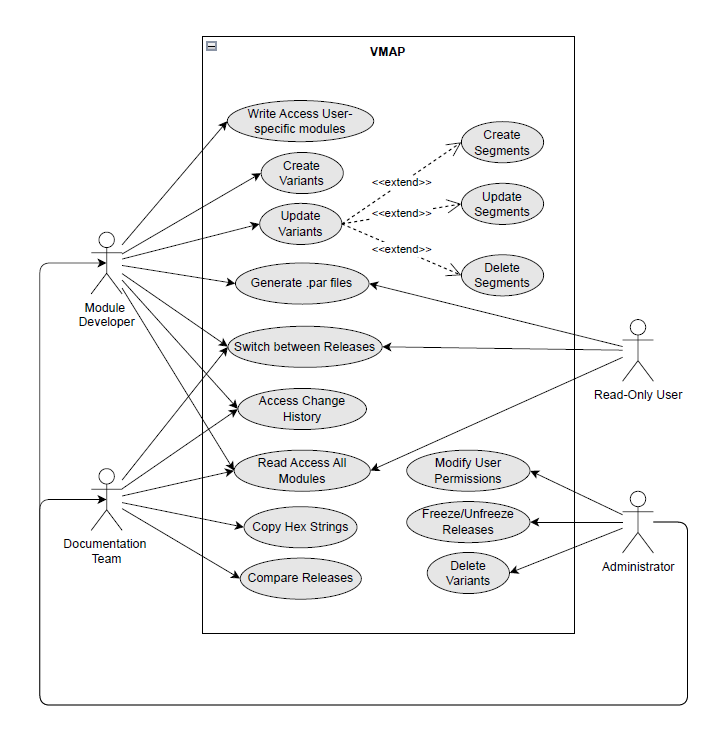
\includegraphics[width=0.95\textwidth]{figures/vmap_use_case_diagram.png}
    \caption{\ac{VMAP} System Use Case Diagram}
    \label{fig:use-case-diagram}
\end{figure}

The use case diagram in Figure \ref{fig:use-case-diagram} illustrates the primary actors and their interactions with the \ac{VMAP} system. Four primary actor types are identified, corresponding to the user roles established during requirements analysis: Module Developers, who create and modify parameter variants; Documentation Team members, who access parameter data for documentation purposes; Administrators, who manage system settings and user access; and Read-Only Users, who view parameter data without making modifications.

This use case model provides a clear visual representation of the system's scope and functionality, serving as a bridge between user requirements and technical implementation. By mapping user roles to specific system functions, the model ensures that the database design will support all required user interactions while maintaining appropriate access controls.

\section{User Management Approaches}
\label{sec:user-management-approaches}

Based on the identified user role requirements, two distinct approaches to user management were considered for the \ac{VMAP} system: a traditional role-based approach and a hybrid role-permission approach. Each approach offers different advantages in terms of flexibility, administrative complexity, and alignment with organizational needs.

\subsection{Traditional Role-Based Approach}
\label{subsec:traditional-role-approach}

\begin{figure}[h]
    \centering
    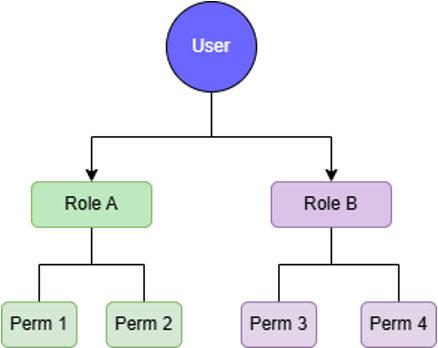
\includegraphics[width=0.7\textwidth]{figures/traditional_rbac_model.png}
    \caption{Traditional Role-Based Access Control Approach}
    \label{fig:traditional-rbac}
\end{figure}

The traditional role-based approach, illustrated in Figure \ref{fig:traditional-rbac}, assigns users to predefined roles that contain fixed sets of permissions, following the classic \ac{RBAC} model described by Sandhu \cite{sandhu1998role}. In this approach, each user is assigned one or more roles, and all permissions are granted through these role assignments without individual permission adjustments.

This approach offers administrative simplicity, as user management involves only assigning appropriate roles rather than configuring individual permissions. The role structure also provides clear organizational alignment, with roles directly corresponding to job functions within the development process. A key limitation is its reduced flexibility for accommodating exceptions or specialized access requirements, potentially compromising the principle of least privilege \cite{sandhu1998role}.

\subsection{Hybrid Role-Permission Approach}
\label{subsec:hybrid-approach}

\begin{figure}[h]
    \centering
    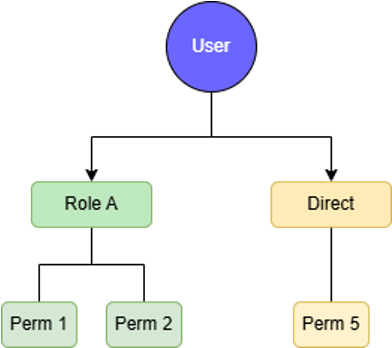
\includegraphics[width=0.7\textwidth]{figures/hybrid_rbac_model.png}
    \caption{Hybrid Role-Permission Access Control Approach}
    \label{fig:hybrid-rbac}
\end{figure}

The hybrid approach, illustrated in Figure \ref{fig:hybrid-rbac}, combines role-based permissions with direct permission assignments, similar to the model described by Ferraiolo et al. \cite{ferraiolo2011policy}. In this approach, users are assigned to primary roles defining their core permissions, but additional permissions can be granted on a per-user basis to address exceptional cases or specialized responsibilities.

This approach offers greater flexibility for accommodating exceptions without creating specialized roles, essential in environments where organizational structures evolve over time. It provides more granular permission control, allowing precise tailoring of access rights to individual responsibilities. However, this flexibility comes at the cost of increased administrative complexity. The hybrid approach is particularly valuable in the automotive parameter management context, where development responsibilities can vary between projects and temporary access adjustments may be needed for specific tasks or during transition periods.

\section{Parameter Synchronization Approaches}
\label{sec:parameter-sync-approaches}

Integration with the \ac{PDD} represents a critical aspect of the \ac{VMAP} system, requiring careful consideration of synchronization approaches. Two different conceptual approaches were explored for maintaining parameter data across the release phases: the change-based approach and the phase-based approach.

\subsection{Change-Based Synchronization Approach}
\label{subsec:change-based-sync}

\begin{figure}[h]
    \centering
    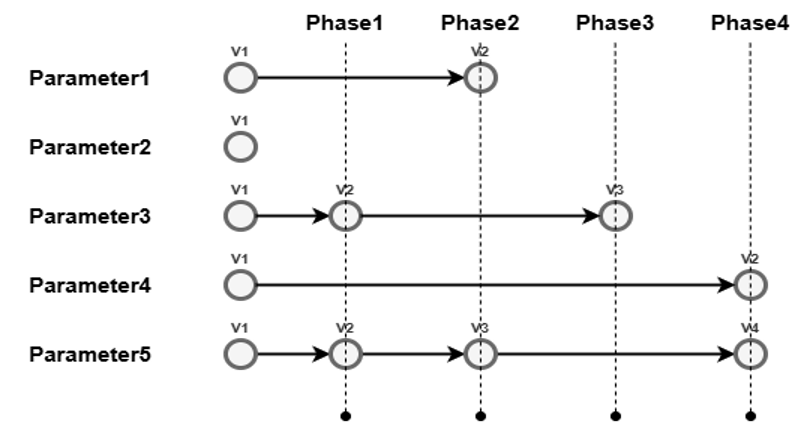
\includegraphics[width=0.95\textwidth]{figures/change_based_approach.png}
    \caption{Change-Based Parameter Synchronization Approach}
    \label{fig:change-based-sync}
\end{figure}

The change-based approach, illustrated in Figure \ref{fig:change-based-sync}, maintains parameter values by recording changes between phases rather than storing complete parameter sets for each phase. Parameters are initially created before the first phase, and subsequent modifications are recorded as change entries associated with specific phases.

This approach is conceptually aligned with traditional version control systems as described by Bhattacherjee et al. \cite{bhattacherjee2015principles}, where efficiency is achieved by storing only the differences between versions rather than complete copies. While potentially offering storage efficiency advantages, this approach introduces conceptual complexity for retrieving parameter values in a specific phase, requiring reconstruction of parameter states from change history.

\subsection{Phase-Based Synchronization Approach}
\label{subsec:phase-based-sync}

\begin{figure}[h]
    \centering
    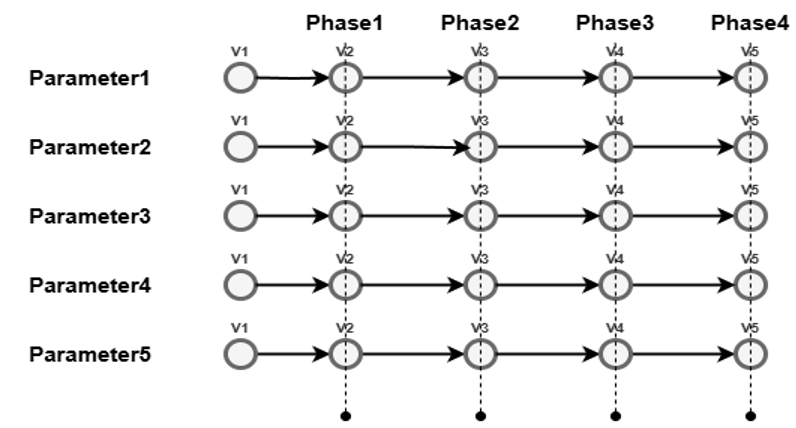
\includegraphics[width=0.95\textwidth]{figures/phase_based_approach.png}
    \caption{Phase-Based Parameter Synchronization Approach}
    \label{fig:phase-based-sync}
\end{figure}

The phase-based approach, illustrated in Figure \ref{fig:phase-based-sync}, maintains complete parameter sets for each phase independently. When parameters are initially created before Phase1, each parameter has its specific version. When transitioning to a new phase, all parameters are copied forward, even if they haven't changed.

This approach aligns more directly with the phase-oriented structure of automotive development described by Broy \cite{broy2006challenges}, where distinct development milestones form the primary organizational principle. The approach simplifies conceptual understanding and parameter retrieval, as parameters for a specific phase can be accessed directly without reconstructing their values from change history.

The phase-based approach also simplifies phase inheritance by copying parameter configurations forward during phase transitions, allowing subsequent modifications in each phase without affecting previous phases. While requiring increased storage due to parameter duplication across phases, this trade-off provides benefits in terms of conceptual clarity, query simplicity, and alignment with the automotive development workflow.

\section{Database System Considerations}
\label{sec:database-system-considerations}

Selecting an appropriate database management system for \ac{VMAP} required consideration of different options against the specific requirements of automotive parameter management. The requirements analysis identified several critical database capabilities needed for effective parameter management: support for complex data types including arrays for multi-dimensional parameters, robust transaction support for maintaining data consistency, advanced indexing capabilities for optimizing common query patterns, extensibility for implementing domain-specific operations, comprehensive access control mechanisms, and efficient storage and retrieval of historical data for audit and traceability purposes.

\begin{table}[htbp]
\centering
\caption{Comparison of Database Systems for Automotive Parameter Management}
\label{tab:database-comparison}
\begin{tabular}{|p{2.5cm}|p{2.5cm}|p{2.5cm}|p{2.5cm}|p{2.5cm}|}
\hline
\textbf{Feature} & \textbf{PostgreSQL} & \textbf{Oracle} & \textbf{SQL Server} & \textbf{MySQL} \\
\hline
\textbf{Complex Data Types} & 
Excellent support for arrays, JSON, custom types \cite{shaik2020postgresql} & 
Good support, additional licensing for advanced features \cite{agarwaloracle} & 
Limited built-in support, extensions required \cite{ward2022sql} & 
Limited support, improved in recent versions \cite{bramer2015web} \\
\hline
\textbf{Transaction Support} & 
Comprehensive with serializable isolation \cite{shaik2020postgresql} & 
Excellent with advanced options \cite{agarwaloracle} & 
Robust support with multiple isolation levels \cite{ward2022sql} & 
Limited in some storage engines \cite{kroghmysql} \\
\hline
\textbf{Indexing Capabilities} & 
Diverse index types including GIN for text search \cite{shaik2020postgresql} & 
Advanced indexing with optimizer hints \cite{agarwaloracle} & 
Solid capabilities with columnstore indexes \cite{ward2022sql} & 
Basic indexing with some limitations \cite{kroghmysql} \\
\hline
\textbf{Extensibility} & 
Highly extensible with custom types and functions \cite{shaik2020postgresql} & 
Extensible with proprietary mechanisms \cite{agarwaloracle} & 
Extensible through .NET integration \cite{ward2022sql} & 
Limited extensibility \cite{bramer2015web} \\
\hline
\textbf{Licensing} & 
Open source, PostgreSQL License \cite{shaik2020postgresql} & 
Commercial, complex licensing model \cite{agarwaloracle} & 
Commercial with edition-based pricing \cite{ward2022sql} & 
Dual licensing: GPL and commercial \cite{bramer2015web} \\
\hline
\end{tabular}
\end{table}

Based on the comparative analysis presented in Table \ref{tab:database-comparison}, PostgreSQL was selected as the database platform for the \ac{VMAP} implementation. This decision was driven by PostgreSQL's native support for arrays, JSON/JSONB, and custom data types, which provides essential capabilities for representing multi-dimensional parameters and complex variant structures \cite{shaik2020postgresql}. PostgreSQL's diverse indexing capabilities, including GIN indexes for full-text search and partial indexes for conditional indexing, provide optimal support for the complex query patterns common in parameter management. The open-source nature of PostgreSQL eliminates licensing costs while providing enterprise-grade capabilities, which was particularly important for the research context of this thesis.

\section{Entity-Relationship Model}
\label{sec:entity-relationship-model}

Based on the requirements analysis and architectural considerations, a comprehensive \ac{ER} model was developed to capture the complex relationships between system entities. This model follows the approach described by Chen \cite{chen1976entity}, providing a conceptual foundation for the database implementation.

\begin{figure}[h]
\centering
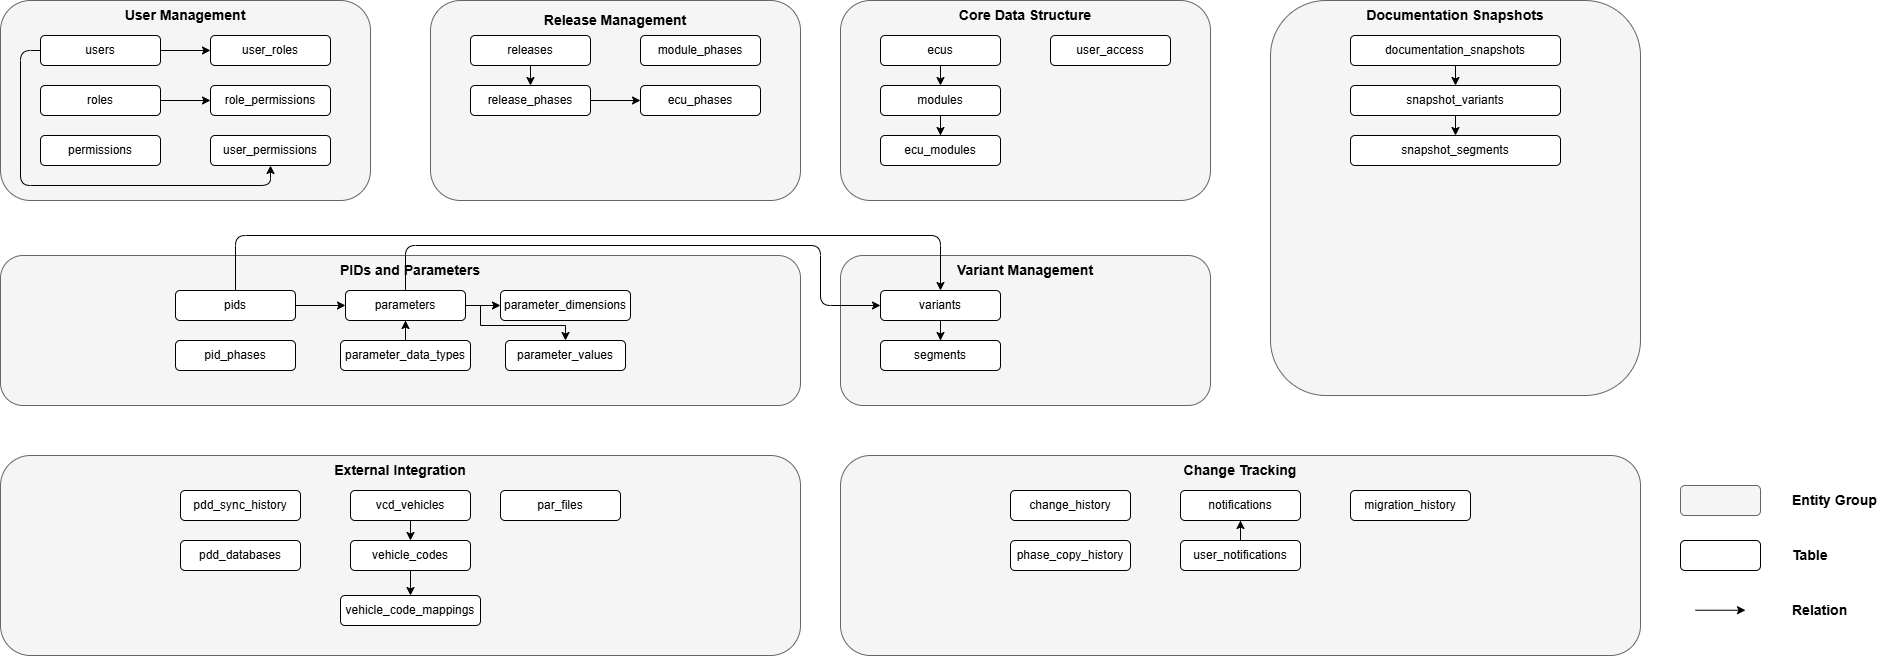
\includegraphics[width=1.0\textwidth]{figures/vmap_er_diagram.png}
\caption{Comprehensive Entity-Relationship Diagram for the \ac{VMAP} System}
\label{fig}
\end{figure}

Figure \ref{fig} illustrates the complete entity-relationship model for the \ac{VMAP} system, showing the logical organization of entities into functional groups and the relationships between them. The diagram captures the hierarchical structure of automotive parameter data, the phase-based versioning approach, the role-permission access control model, and the mechanisms for external system integration and change tracking.

\subsection{Core Data Entities}
\label{subsec:core-data-entities}

The \ac{ER} model includes several categories of entities representing different aspects of the system. User management entities include Users, Roles, Permissions, and their relationships, implementing a role-permission model for access control. Release management entities encompass Releases, Release Phases, and \ac{ECU} Phase mappings, providing the foundation for the phase-based version control approach. Parameter structure entities include \acp{ECU}, Modules, \acp{PID}, Parameters, and Parameter Dimensions, representing the hierarchical organization of vehicle electronic systems as described by Staron \cite{staron2021automotive}.

Variant management entities comprise Variants, Segments, and their relationships to parameters, implementing the core parameter customization functionality. Documentation entities include Documentation Snapshots, Snapshot Variants, and Snapshot Segments, supporting the preservation of historical parameter states for documentation and regulatory compliance. Integration entities consist of Synchronization Records, Vehicle Configurations, and Parameter File Records, supporting connectivity with external systems. Audit entities encompass Change History, Transaction Records, and Phase Copy History, providing comprehensive traceability for all significant operations within the system.

\subsection{Relationship Structure}
\label{subsec:relationship-structure}

The relationships between entities in the \ac{ER} model reflect the complex interactions between different aspects of automotive parameter management. Key relationships include hierarchical relationships between \acp{ECU}, Modules, \acp{PID}, and Parameters, representing the structural organization of automotive electronic systems. Many-to-many relationships between parameters and phases are implemented through direct association rather than temporal versioning, supporting the phase-based versioning approach and allowing efficient retrieval of parameters for specific phases.

Complex relationships between variants, parameters, and segments capture the parameter customization process, ensuring that segments are associated with valid variants and parameters while supporting efficient resolution of effective parameter values based on vehicle configuration. Temporal relationships for audit and history entities capture the evolution of parameter configurations over time, supporting both regulatory compliance and diagnostic capabilities.

The \ac{ER} model was developed using data normalization principles to minimize redundancy while maintaining data integrity, following the approach described by Codd \cite{codd1970relational}. The model generally adheres to \ac{3NF}, ensuring that non-key attributes depend on the primary key rather than on other non-key attributes. Strategic denormalization was considered in specific areas to optimize performance for common operations, following the principles described by Churcher \cite{churcher2008beginning}.

\section{Validation Mechanisms}
\label{sec:validation-mechanisms}

To ensure data integrity and consistency, multiple validation mechanism layers were conceptualized for the \ac{VMAP} system, from basic constraints to sophisticated business rule validation. These mechanisms work together to maintain parameter data quality and reliability throughout the system lifecycle.

Database-level constraints form the foundation for enforcing basic integrity rules, following the principles described by Sciore \cite{sciore2009database}. These constraints include primary key constraints ensuring unique entity identifiers, foreign key constraints maintaining referential integrity between related entities, not-null constraints ensuring required fields contain values, unique constraints preventing duplicate values in specified columns, and check constraints enforcing domain-specific rules such as valid date ranges and parameter value ranges.

Domain-specific business rules are implemented through database triggers and stored procedures, providing a second layer of validation beyond basic constraints. These rules include parameter range validation automatically checking modified values against defined minimum and maximum bounds, phase status validation preventing modifications to frozen phases, segment validation ensuring segments reference valid parameters and variants, and user access validation ensuring users can only modify parameters, variants, and segments for modules to which they have been granted access.

Comprehensive audit and traceability mechanisms are essential for regulatory compliance and quality assurance in automotive parameter management. The core of this capability is the change history tracking mechanism, which automatically captures both before and after states for entity modifications. For each change, the system records the entity being modified, the type of change, the user making the change, the timestamp, and detailed before/after values. To optimize performance, selective filtering of change data excludes non-essential fields such as timestamps and large binary data, while asynchronous audit recording for bulk operations reduces the performance impact on high-volume operations while ensuring that all changes are eventually recorded.